\documentclass[12pt,letterpaper]{article} % a. Set paper size to Letter, 8½ x 11. 

% TODO: change author's name in settings
\input{settings}

\begin{document}

% TODO: decide on used language
%\selectlanguage{english}
\selectlanguage{german}

% TODO: change thesis information

\begin{center}\uppercase{Ludwig-Maximilians-Universität München}\end{center}
\iflanguage{english}{
\begin{center}\uppercase{Chair of Theoretical Computer Science and Theorem Proving}\end{center}
}
{}
\iflanguage{german}{
\begin{center}\uppercase{Lehr- und Forschungseinheit für Theoretische Informatik und Theorembeweisen}\end{center}
}
{}

\vspace*{10mm}
\begin{center}
\includegraphics[height=40mm]{sigillum.png}
\end{center}
\vspace*{10mm}

% TODO: decide if english or german

\iflanguage{english}{
%%%Block Englisch:
\title{Thesis Title}
\date{\vspace{-3ex}}
{\let\newpage\relax\maketitle}
\thispagestyle{empty}

\begin{center}
\begin{large}
\begin{Large}
Bachelorarbeit im Studiengang Informatik mit integriertem Anwendungsfach Computerlinguistik\\
\end{Large}
in course type (Computer Science, Computer Science plus Mathematics, \ldots) \\
\end{large}
\end{center}
\vspace{1cm}
\begin{center}
\begin{large}
Supervisor: Prof. Dr. Jasmin Blanchette\\
\end{large}
\end{center}
\begin{center}
\begin{large}
Advisor: Advisor's name\\
\end{large}
\end{center}
%%%Ende Block Englisch
}{}

\iflanguage{german}{
%%%Block Deutsch:
\title{Titel der Arbeit}
\date{\vspace{-5ex}}
{\let\newpage\relax\maketitle}
\thispagestyle{empty}
\begin{center}
\begin{large}
\begin{Large}
Bachelorarbeit\\
\end{Large}
im Studiengang Informatik mit integriertem Anwendungsfach Computerlinguistik\\
\end{large}
\end{center}
\vspace{1cm}
\begin{center}
\begin{large}
Betreuer: Prof. Jasmin Blanchette\\
\end{large}
\end{center}
\begin{center}
\begin{large}
Mentor: Balazs Toth\\
\end{large}
\end{center}
%%%Ende Block Deutsch
}{}

\begin{center}
\begin{large}
\iflanguage{english}{
Submission Date: \date{\today} \\
}
{}
\iflanguage{german}{
Ablieferungstermin: \date{\today} \\
}
{}
\end{large}
\end{center}

\vspace{1,5cm}
\input{pages/disclaimer}
\thispagestyle{empty}

\vspace*{20mm}

\begin{center}
\makeatletter

\iflanguage{english}{
{\normalfont\bfseries} Acknowledgments
}
{}
\iflanguage{german}{
{\normalfont\bfseries} Danksagungen
}
{}
\makeatother
\end{center}

\vspace{10mm}
Ich möchte die Gelegenheit nutzen und mich bei allen bedanken, die mich bei dem Entwurf dieser Bachelorarbeit unterstützt haben.

Zuallererst möchte ich Prof. Dr. Jasmin Blanchette für die Bewertung meiner Bachelorarbeit und für die aufschlussreichen Ratschläge und die konstruktive Kritik bedanken, die ich zu Beginn dieser Arbeit und während meines Antrittsvortrags erhalten habe.

Außerdem möchte ich mich herzlich bei Balazs Toth, meinem Mentor, bedanken, der mir während der Entwicklung des Programms und des gesamten Schreibprozesses konstruktive Kritik und Unterstützung gegeben hat.

Ich möchte mich auch bei Fabian Huch, dem Entwickler von FindFacts, für seine Hilfe und Ratschläge bedanken.

Darüber hinaus möchte ich meiner Familie und meiner Freundin für ihre Motivation sowie für ihre Unterstützung beim Korrekturlesen danken.
\cleardoublepage{}
 % TODO: if you don't have anyone to thank for or don't wish to publish it, comment this line out.
% TODO: decide if english or german
\iflanguage{english}{
\section*{Abstract}
}
{}
\iflanguage{german}{
\section*{Kurzfassung}
}
{}
Die vorliegende Bachelorarbeit befasst sich mit der Entwicklung einer KI-gestützten semantischen Suche von Theoremen in Isabelle/HOL und dem Archive of Formal Proofs und dessen Evaluation.

Die steigende Anzahl an formalen Bibliotheken erschwert die manuelle Suche nach Theoremen.
Zudem ist die Wiederverwendung bestehender Theoreme essenziell, um Duplikate zu vermeiden.
Nutzer bestehender Suchmaschinen haben außerdem berichtet, dass sie es als schwierig empfinden zu prüfen ob ein Theorem im Archive of Formal Proofs bereits exisitiert.

Gleichzeitig stellen transformerbasierte Sprachmodelle eine vielversprechende Technologie für semantische Suchmaschinen dar.

\textbf{Keywords}: Artificial Intelligence, Healthcare Delivery, Patient Care, Diagnostic Accuracy, Treatment Optimization, Ethical Considerations, Regulatory Frameworks.


\newpage
\tableofcontents
\newpage

\setcounter{page}{1}
\pagestyle{fancy}
\fancyhf{}
\fancyhead[R]{\thepage}
\renewcommand{\headrulewidth}{0pt} %obere Trennlinie

%OUTLINE%
\section{KI-gestützte Theoremsuche in Isabelle: Ein transformerbasierter Ansatz}

\section{Einleitung}

\subsection{Motivation und Problemstellung}
- Isabelle: generischer interaktiver Theorembeweiser mit besonderem Schwerpunkt auf Higher-Order Logic\\
- formale Verifizierung von Hard- und Software\\
- AFP: peer-reviewte Datenbank von Beweisbibliotheken\\
- stetig wachsende Zahl an Einträgen und formalen Theoremen im AFP (Quelle: Mining the Archive of Formal Proofs", https://www.isa-afp.org/statistics/ **(Frage: Darf ich die Statistik mit der Anzahl der Theoreme im AFP zitieren?)**)\\
- Wiederverwendung bestehender Theorem essenziell um Duplikate zu vermeiden $\rightarrow$ zu wenig (Quelle: Mining the Archive of Formal Proofs" > Conclusion)\\
- Suchmaschinen wie isa-afp.org oder FindFacts oder Befehle wie find theorems oder grep erlauben nur lexikalische Suche $\rightarrow$ keine Semantische Suche\\
- Keine Treffer bei abweichenden Begriffen oder Reihenfolge der Begriffe\\
- Keine Ähnlichkeitserkennung oder intelligentes Ranking der Suchergebnisse\\
- Schwierig für Nutzer bestehende Theoreme wieder zu finden\\
- gleichzeitig aber: Potential aktueller KI-Modelle für semantisches Retrieval

\subsection{Zielsetzung}
- Ziel: Entwicklung und Evaluation einer KI-gestützten semantischen Suche nach Theoremen, Lemmas und Corollaries im AFP\\
- Verwendung vortrainierter Transformer-Modelle in Form von LLM zur Textgenerierung von Theorem-Beschreibungen und Optimieren einer Suchanfrage, Bi-Encoder zur Ähnlichkeitssuche und ChromaDB zur effizienten Speicherung und Vektorsuche\\
- Vergleich verschiedener Suchstrategien wie LLM-Umschreibung von Suchanfragen oder Metadatenintegration, anschließende Evaluation und Analyse durch Benchmark\\
- *(optional: Entwicklung der restAPI und Webseite, Docker-Container...?)*

\subsection{Forschungsfragen}
- Wie effektiv sind LLMs bei der Umschreibung von formalen Theoremen, um deren Auffindbarkeit durch Suchanfragen des Nutzers zu verbessern?\\
- Wie wirkt sich das Optimieren einer Suchanfrage durch LLMs oder das Einbetten von Metadaten eines entsprechenden Theorems, wie Titel oder Abstract des Entries, auf die Suchqualtität aus?\\
- Wie effektiv ist die Theoremsuche laut des Benchmarks und wie robust ist sie gegenüber simulierten Fehlern bei Suchanfragen?

\subsection{(optional: Aufbau?)}


\section{Hintergrund}

\subsection{Isabelle, AFP und formale Beweise}
- **(Frage: Soll ich mich hier wiederholen? Ich erkläre in *Motivation und Problemstellung* ja schon, was das AFP und Isabelle ist)**\\
- Isabelle\\
- AFP: besteht aus Entries, die aus formalen Theoremen, Definitionen, Beweisen, etc. bestehen\\
- außerdem: Paper mit Title, Abstract

\subsection{Bestehende Suchmechanismen}
- **(Frage: Soll ich mich hier wie oben wieder wiederholen)**\\
- FindFacts, isa-afp.org, find theorem, grep?\\
- Was ist FindFacts? Wie funktioniert die bisherige Suche?\\
- aber: unterstützen jeweils nur lexikalische Suche, keine Semantische Suche

\subsection{Transformerbasierte Sprachmodelle}
- **(Frage: soll ich Transformer "from scratch" erklären oder ist das zu viel?)**

\subsection{ChromaDB}
- **(Frage: soll ich ChromaDB erklären oder nur kurz erwähnen/erklären?)**\\
- z.B. "https://aclanthology.org/2024.findings-emnlp.470.pdf" geht nur kurz darauf ein\\
- Ich persönlich finde fast, dass ein eigenes Unterkapitel zu viel dafür ist :)

\subsection{Verwandte Arbeiten}
- $Gao, G., Ju, H., Jiang, J., Qin, Z., \and Dong, B. (2024). A semantic search engine for Mathlib4. arXiv preprint arXiv:2403.13310.$\\
- Huch, F., \and Krauss, A. (2022). FindFacts: a scalable theorem search. arXiv preprint arXiv:2204.14191.\\
- genügen 2 Verwandte Arbeiten?


\section{Methodik}

\subsection{Programmaufbau}
- Detaillierte Schritt-für-Schritt Erklärung des Programm-Ablaufs, z.B.:\\
- benötigt fertigen FindFacts-Index, d.h. baut darauf auf\\
- verbindet sich mit bereits laufender Solr-Datenbank\\
- lädt aus der Solr-DB nur Dokumente mit dem "command" theorem/lemma/corollary\\
- prüft für jedes Theorem, ob dieses bereits vom in der config festgelegten LLM beschrieben informalisiert wurde \\
- auch z.B. auf Caching und Standard-Konfiguration eingehen\\
- Generierte LLM-Outputs werden gespeichert und können committet werden, um zu verhindern, das andere Nutzer die selben Outputs nochmal generieren müssen \\
- ...\\
- bei einer Suchanfrage: LLM umschreibt die Suchanfrage, um die Suchqualität zu verbessern (optional und kann deaktiviert werden)\\
- startet Flask-API-Server zur Bereitstellung einer REST-API

\subsection{Informalisierung der Theoreme}
- was ist "Informalisierung" der Theorem?
  - $\rightarrow$ LLM umschreibt den Theorem-Code in informale Sprache, damit es leichter zum Finden ist\\
- warum ausgerechnet das LLM microsoft/Phi-3.5-mini-instruct?
  - $\rightarrow$ technische Limitationen
  - $\rightarrow$ Wahl anhand von LLM Leaderboard\\
- Beispiel: Prompt, Input Theorem, Umschreibung\\
- **(Frage: Prompt-Beispiel lieber hier oder in den Anhang mit Referenz?)**


\section{Benchmark}

\subsection{Aufbau des Benchmarks}
- Quelle: Freek's "Top 100 Theorems in Isabelle"\\
- Struktur der Benchmark-Tabelle: ID, Title, Theorem, Target Identifiers, Link, Session, Annotation als CSV *(soll ich jede column erklären?)*\\
- Generierung der Queries: Title, Natural language query, noisy natural language query\\
- Erklärung der Query-Arten und wie sie erstellt wurden (z.B. Zitat aus Wikipedia)\\
- Beispiel für Query Arten und Ziel Theoreme

\subsection{Benchmark-Pipeline und Vergleich der Suchstrategien}
- Ablauf des Benchmarks erklären\\
- Verschiedene Suchstrategien erklären:
  - Theorem-Embeddings ohne Metadaten + LLM-Suchanfragen-Umschreibung 
  - Theorem-Embeddings mit Metadaten + LLM-Suchanfragen-Umschreibung 
  - Theorem-Embeddings ohne Metadaten ohne LLM-Suchanfragen-Umschreibung 
  - Theorem-Embeddings mit Metadaten ohne LLM-Suchanfragen-Umschreibung
  - Theorem-Embeddings ohne Metadaten + Hybrid (Query + LLM-Suchanfragen-Umschreibung)
  - Theorem-Embeddings mit Metadaten + Hybrid (Query + LLM-Suchanfragen-Umschreibung)

\subsection{Verwendete Metriken}
- jede Metrik als Formel erklären $\rightarrow$ was sagt diese Metrik aus?


\section{Ergebnis und Analyse}

\subsection{Vergleich der Suchstrategien}
- Beste Strategie: Ohne Metadata + Hybrid Queries.\\
- jeden Query-Typ auswerten, d.h. die durchschnittlichen gemessenen Werte für jede Metrik für jede Query beschreiben

\subsection{Erklärung von Performance-Unterschieden}
- Einfluss von Metadaten und Query Refinement\\
- Beispiel\\
- Metadaten machen Suche schlechter\\
- Beispiel\\
- Refined Queries helfen\\
- Beispiel\\
- LLM tendiert zur Reproduktion von Train-Prompts bei langen Prompts (schwer zu erklären, warum)\\
- wenn die LLM-Umschreibung von Suchanfragen falsch ist sind die Ergebnisse fast immer falsch/schlecht $\rightarrow$ Beispiel


\section{Limitationen}
- Benchmark hardware-technisch beschränkt (GPU hat nicht genug VRAM oder Modelle wie DeepSeek sind laut LLM Benchmark sehr gut aber zu groß)\\
- Programm funktioniert schlecht auf ressourcenbeschränkten Geräten (z.B. Laptops)\\
- Die LLM-Umschreibung zu deaktivieren reduziert die Suchzeit erheblich und kann auf ressourcenbeschränkten Geräten helfen, reduziert aber auch die Suchqualität **(Frage: Soll ich hier fixe Werte z.B. 1,9 Sekunden Suchzeit nennen, auch wenn sie eigentlich hardware-abhängig und damit nicht konsistent sind?)**\\
- Benchmark nur von einer Person annotiert/erstellt $\rightarrow$ Risiko von Bias oder Fehlern\\
- wenn die LLM-Umschreibung von Suchanfragen falsch ist sind die Ergebnisse fast immer falsch


\section{Zusammenfassung und Ausblick}
- Zusammenfassung\\
- Idee für Zukunft: Nutzer bei Suchergebnissen fragen "sind diese Ergebnisse hilfreich?" $\rightarrow$ sowohl als Trainingsdaten um Bi-Encoder zu erweitern oder tatsächliche Suchqualität außerhalb des Benchmarks zu überprüfen\\
- KI-Suche kann z.B. in CI/CD-Pipelines oder pre-commit-hooks verwendet werden, um frühzeitig duplizierte Theoreme zu erkennen (im AFP gibt es schon einige Duplikate)


\section{Literaturverzeichnis}
%END_OUTLINE%

\section{Introduction}
This document serves as a template for bachelor or master theses in the 'Chair of Theoretical Computer Science and Theorem Proving' at \gls{lmu}. 
By commenting one of the commands $selectlanguage\{english\}$ or $selectlanguage\{german\}$ the documents language is changed.
\\ To build the main version run the command \texttt{make} in the terminal.
\\The template follows the guidelines of the journal \emph{language} (\url{http://www.linguisticsociety.org/sites/default/files/style-sheet.pdf}).

\section{Notes on form}
\subsection{Formatting} 

This LaTeX template uses the following formatting:
\begin{itemize}
\setlength{\itemsep}{0pt}
	\item font: Linux Libertine O (alternatively: Times New Roman)
	\item font size: 12 pt
	\item left and right margin: 3.5 cm, top and bottom margin: 3 cm
    \item align: left
	\item line spacing: one and a half (alternative: 15 pt line spacing with 12 pt font size)
\end{itemize}

\noindent
When implementing the specifications in Word, it is essential to define style sheets.

\subsection{Citation} 
\label{sec:cit}

The citation method follows the author-year system. Place reference is in the text, footnotes should only be used for explanations and comments. The following notes are taken from the \emph{language} bibliography template from \url{ron.artstein.org}:\newline

\noindent
The \emph{Language} style sheet makes a distinction between two kinds of in-text citations: citing a work and citing an author.
\begin{itemize}
\item Citing a work:
  \begin{itemize}
    \setlength{\itemsep}{0pt}
    \setlength{\parsep}{0pt}
  \item Two authors are joined by an ampersand (\&).
  \item More than two authors are abbreviated with \emph{et al.}
  \item No parentheses are placed around the year (though parentheses
    may contain the whole citation). 
  \end{itemize}
\item Citing an author:
  \begin{itemize}
    \setlength{\itemsep}{0pt}
    \setlength{\parsep}{0pt}
  \item Two authors are joined by \emph{and}.
  \item More than two authors are abbreviated with \emph{and colleagues}.
  \item The year is surrounded by parentheses (with page numbers, if
    present).
  \end{itemize} 
\end{itemize}
To provide for both kinds of citations, \verb+language.bst+ capitalizes on the fact that \verb+natbib+ citation commands come in
two flavors. In a typical style compatible with \verb+natbib+, ordinary commands such as \verb+\citet+ and \verb+\citep+ produce short
citations abbreviated with \emph{et al.}, whereas starred commands such as \verb+\citet*+ and \verb+\citep*+ produce a citation with a
full author list. Since \emph{Language} does not require citations with full authors, the style \verb+language.bst+ repurposes the starred commands to be used for citing the author. The following table shows how the \verb+natbib+ citation commands work with \verb+language.bst+.
\begin{center}
  \begin{tabular}{lll}
    \toprule
    Command & Two authors & More than two authors \\
    \midrule
    \verb+\citet+ & \citet{hale} & \citet{sprouse} \\
    \verb+\citet*+ & \citet*{hale} & \citet*{sprouse} \\
    \addlinespace
    \verb+\citep+ & \citep{hale} & \citep{sprouse} \\
    \verb+\citep*+ & \citep*{hale} & \citep*{sprouse} \\
    \addlinespace
    \verb+\citealt+ & \citealt{hale} & \citealt{sprouse} \\
    \verb+\citealt*+ & \citealt*{hale} & \citealt*{sprouse} \\
    \addlinespace
    \verb+\citealp+ & \citealp{hale} & \citealp{sprouse} \\
    \verb+\citealp*+ & \citealp*{hale} & \citealp*{sprouse} \\
    \addlinespace
    \verb+\citeauthor+ & \citeauthor{hale} & \citeauthor{sprouse} \\
    \verb+\citeauthor*+ & \citeauthor*{hale} & \citeauthor*{sprouse} \\
    \verb+\citefullauthor+ & \citefullauthor{hale} & \citefullauthor{sprouse} \\
    \bottomrule
  \end{tabular}
\end{center}
Authors of \emph{Language} articles would typically use \verb+\citet*+, \verb+\citep+, \verb+\citealt+ and \verb+\citeauthor*+, though they
could use any of the above commands. There is no command for giving a full list of authors.

\subsection{Bibliography}
The bibliography of this template includes the references of the \emph{language} stylesheet as a sample bibliography.

\pagebreak

% TODO: appendix chapter
\section{Appendix}

\subsection{Anhang 1: Screenshot der Webseite}

\begin{figure}[!htb]
  \centering
  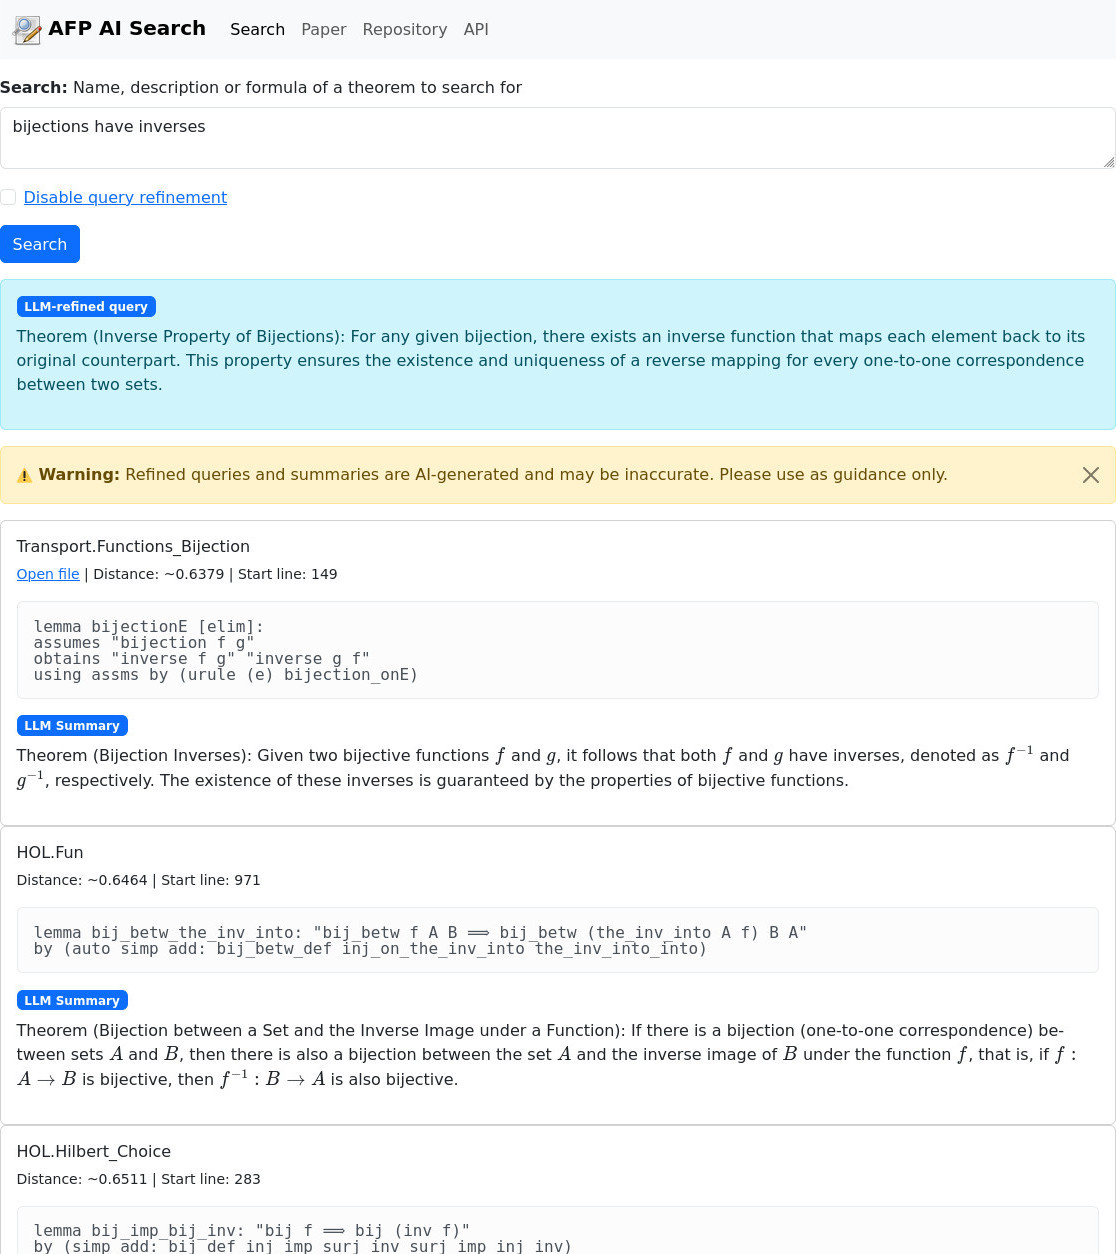
\includegraphics[width=\textwidth]{website_screenshot.jpg}
  \caption{Screenshot der Webseite}
\end{figure}


\pagebreak

\microtypesetup{protrusion=false}
\listoffigures{}
\listoftables{}
\microtypesetup{protrusion=true}

\clearpage
\printglossaries

\pagebreak

\iflanguage{english}{
\addcontentsline{toc}{section}{Bibliography}
}
{}
\iflanguage{german}{
\addcontentsline{toc}{section}{Literatur}
}
{}
\pagestyle{fancy}

\bibliographystyle{language-dt} %using language.bst
\bibliography{bibliography} %bib-filename

\nocite{*} %List all bib-entries

\end{document}
